\chapter{Uvod}

\qquad U ovom radu je predstavljeno upravljanje električnim vozilom (slika \ref{fig:buggy}) sa pogonom na sva četiri točka. Proizvođač \href{https://www.qsmotor.com/product/8000w-car-motor/}{motora} je kompanija \textit{QSMOTOR}. Snaga motora je $8000W$, a standardni napon napajanja iznosi $72V$. Svaki od motora je spojen na odgovarajući pretvarač/\href{https://kellycontroller.com/shop/kls-h/}{invertor}. Motori su trofazni i sadrže dva seta Hallovih senzora za određivanje brzine i pozicije. Datasheet motora je dat u prilogu \ref{motor_datasheet}, a dio dokumentacije pretvarača \textit{KLS7275H} u prilogu \ref{kelly_datasheet}. Razvoj upravljačkog prototipa će biti realiziran pomoću \href{https://www.dspace.com/en/inc/home/products/hw/microlabbox.cfm?fbclid=IwAR08_hHwsXPVRs6ng2DLSU5HA3vDNzpBa9CMpO8DWlSQ1DXPK58BkLmoiRE}{dSpace} sistema.

\section{Motor}

\qquad Motor je trofazni sa $16$ pari polova, nominalne snage $8000W$. Za mjerenje brzine i pozicije motora, dostupna su dva seta Hallovih senzora. Moguće je mjeriti i temperaturu motora pomoću temperaturnog senzora $KTY83/122$.

\section{Pretvarač}

\qquad Energetski pretvarač \textit{KLS7275H} proizvođača \textit{Kelly} sadrži 5 digitalnih ulaza: prekidače za gas i kočnicu, prekidače za kretanje naprijed i nazad, te prekidač za \textit{boost} način rada. Dostupna su 3 analogna ulaza: gas, kočnica i temperatura motora. Opseg ulaznog napona može varirati od $0$ do $5V$. Za upravljanje je moguće koristiti i palicu (\textit{engl. joystick}), pri čemu pozicija palice određuje zadanu brzinu i smjer kretanja. \textit{Cruise} režim rada, koji je također dostupan, podrazumijeva zadržavanje zadane brzine vrtnje motora sve dok se ne zada nova brzina ili aktivira kočnica. Pretvarač podržava povezivanje putem \textit{CAN} mreže.

\begin{figure}
\begin{center}
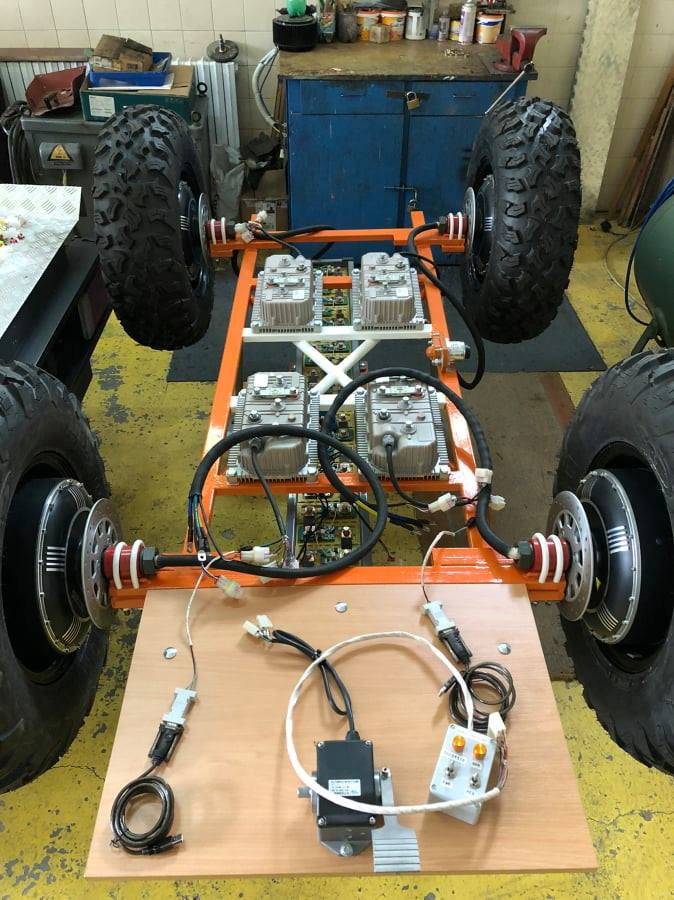
\includegraphics[scale=0.5]{slike/electric_car.jpg}
\end{center}
\caption{Električno $4x4$ vozilo}
\label{fig:buggy}
\end{figure}










